\documentclass{article}

% set font encoding for PDFLaTeX, XeLaTeX, or LuaTeX
\usepackage{ifxetex,ifluatex}
\newif\ifxetexorluatex
\ifxetex
  \xetexorluatextrue
\else
  \ifluatex
    \xetexorluatextrue
  \else
    \xetexorluatexfalse
  \fi
\fi

\ifxetexorluatex
  \usepackage{fontspec}
\else
  \usepackage[T1]{fontenc}
  \usepackage[utf8]{inputenc}
  \usepackage{lmodern}
\fi

\usepackage{hyperref}
\usepackage{graphicx}

\title{Actividad 10}
\author{Jesús Adrián Zatarain Alvarado}

% Enable SageTeX to run SageMath code right inside this LaTeX file.
% http://mirrors.ctan.org/macros/latex/contrib/sagetex/sagetexpackage.pdf
% \usepackage{sagetex}

\begin{document}
\maketitle

\section{Introducción}

Para esta actividad de pide revisar y reproducir el artículo de Geoff Boeing, donde habla acerca de los sistemas no-lineales dinámicos y los sistemas caóticos, estos últimos con más abundancia. Se interpretarán las características de cada uno y se apoyará con gráficas para verificar e interiorizar mejor los conceptos explicados en el artículo.

En el artículo se habla que se desarrolló usando Phyton, para esta ocasión se hará uso de Maxima para realizar lo correspondiente.

La teoría del caos es una rama de las matemáticas que trata con sistemas no lineales dinámicos. Los sistemas caóticos son un subtipo simple de sistemas no lineales dinámicos.

\section{El mapa logístico}

Para representar eñ caos, se puede hacer uso de un mapa logístico. El mapa tiene la particularidad de que está basado en la curva más común que muestra cómo la población crece, para crecer tiempo después más rápidamente y llega a una capacidad constante. El mapa logístico utiliza una ecuación no lineal que toma pasos de tiempo discretos:

\begin{ecuation}

x_t_+_1=rx_t(1-x_t)

\end{ecuation}

La ecuación va a decir cómo va a funcionar el sistema. La x representa la razón de creciecimiento , es decir, el nivel de crecimiento de la población en cualquier momento dado como función del parámetro de la razón de crecimiento y el anterior tiempo de ésta. 

\section{Comportamiento del sistema y atractores}

En el mundo real se puede observar el comportamiento de una población y estudiarla.

En la siguiente gráfica se puede observar cómo la población cambia con respecto al tiempo, dando así diferentes razones de crecimiento.

\begin{center}
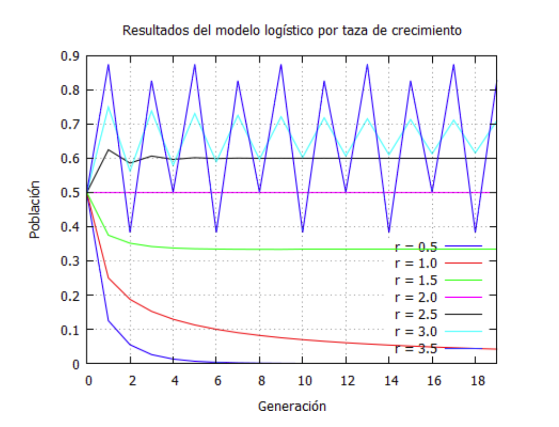
\includegraphics[width=6cm, height=6cm]{Im1.png}
\end{center}

La línea azul representa una tasa de crecimiento de 0.5, y rápidamente cae a cero. La población muere. La línea cian representa una tasa de crecimiento de 2.0 (recuerde, la tasa de reemplazo) y se mantiene estable a un nivel de población de 0.5. Las tasas de crecimiento de 3.0 y 3.5 son más interesantes. Mientras que la línea amarilla para 3.0 parece estar convergiendo lentamente hacia un valor estable, la línea gris para 3.5 solo parece rebotar.

Un atractor es un valor que el sistema lo establece con el tiempo. El valor de la población se dibuja hacia 0 en el tiempo a medida que el modelo se repite.


Pero cuando ajustamos el parámetro de la tasa de crecimiento más allá de 3.5, vemos el inicio del caos. Un sistema caótico tiene un atractor extraño, alrededor del cual el sistema oscila para siempre, nunca se repite o se establece en un estado estable de comportamiento. Nunca golpea el mismo punto dos veces y su estructura tiene una forma fractal, lo que significa que existen los mismos patrones en todas las escalas, sin importar cuánto se acerque a ella.


\section{Bifurcaciones y el camino a la teoría del caos}

Esta vez se va a hacer un modelo para 200 generaciones y variarlas entre razones de 1000 poblaciones entre 0 y 4, para ver cómo se utilizan los diagramas de bifurcación. Estos diagramas son un resumen visual de la sucesión de los valores de la población mientras r aumenta.

\begin{center}
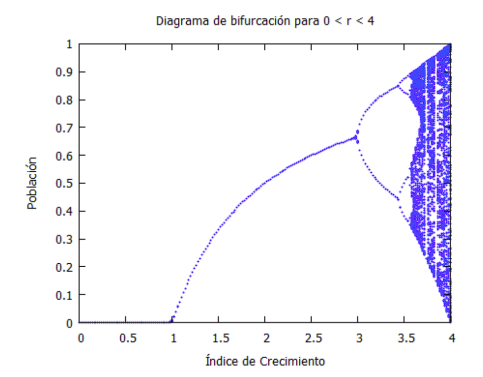
\includegraphics[width=6cm, height=6cm]{Im2.png}
\end{center}

Se uso la fución orbits del paquete de wxMaxima llamado Dynamics, el cual permite generar datos y graficarlos dependiendo de la función que se utilice. Entre 1 y 3, el sistema corresponde a una población estable. Entre 2.8 y 4 está en dos caminos discretos la población. E sistema oscila entre dos valores, 0.5 y 0.8. Se llama diagrama de bifurcación debido a que  aplicando la ecuación logística a uno de esos valores, se obtiene el otro.  y se va a dividir de nuevo en los valores de 3.4, 3.5.

En valores menores que uno, el sistema siempre colapsa a cero, se extingue la población. 
\begin{center}
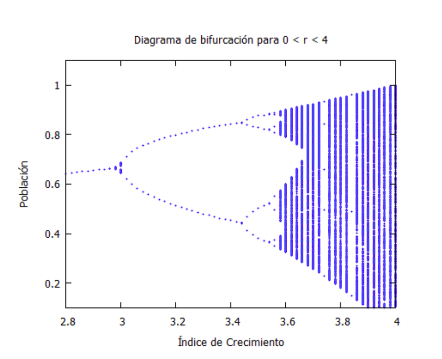
\includegraphics[width=6cm, height=6cm]{Im3.png}
\end{center}






\section{El comienzo de la teoría del caos}

Una vez alcanzada la raza de crecimiento de 3.6, las bifurcaciones aumentan hasta que el sistema es capaz de caer en cualquier valor de la población, a ello se le llama bifurcación del pediodo-doble. Mientras más se cambie el parámetro r, el mapa logístico variará en múltiplos de dos sucesivamente.

\begin{center}
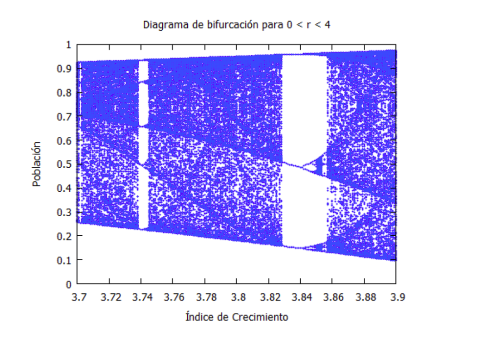
\includegraphics[width=6cm, height=6cm]{Im4.png}
\end{center}

Cuando se alcanza el valor de 3.9, el sistema parece saltar de una manera entre todos los valores que puede tomar la población.  El caos observado es determinista y aperiódico.

\section{Fractales y atractores extraños}

Los sistemas caóticos tienen atractores extraños, los cuales pueden ser caracterizados como fractales.Esto significa que son similares entre ellos, tienen la misma estructura a cualquier escala. Esto se puede observar al hacer un acercamiento en la taza de bifurcación de 3.85.

\begin{center}
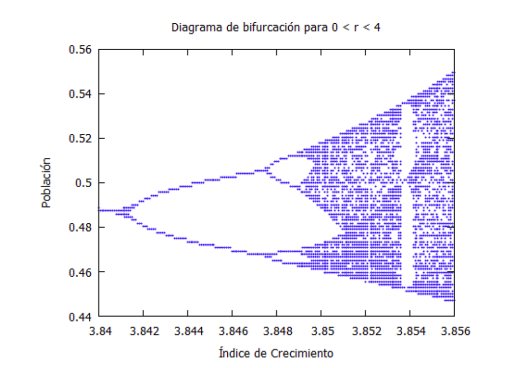
\includegraphics[width=6cm, height=6cm]{Im5.png}
\end{center}

Se puede utilizar un diagrama de fase para visualizarlo. Se grafica la población t+1 en el eje y, contra la población en el valor t en el eje de las x. El valor de la población es constante. 

\begin{center}
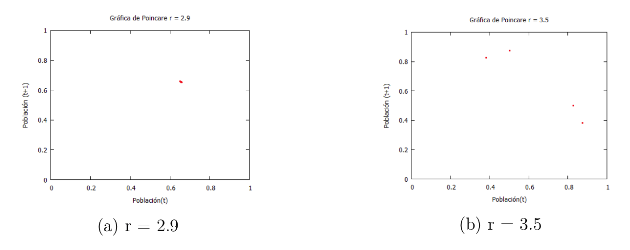
\includegraphics[width=6cm, height=6cm]{Im6.png}
\end{center}

Si se tienen varias difracciones, se muestra una serie de puntos que forman una parábola. El régimen caótico es cuando se llegan a valores de r que no se sobreponen.

\begin{center}
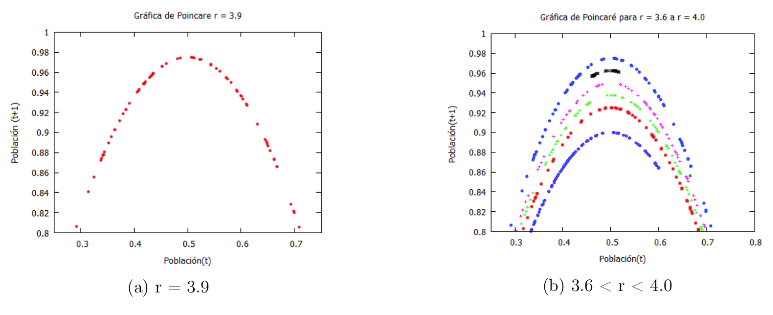
\includegraphics[width=6cm, height=6cm]{Im7.png}
\end{center}

\section{Caos versus aletoridad}

Se presentan ambientes donde no se puede diferenciar si se está trtando con sistemas caóticos o números aleatorios en sistemas dinámicos.

\begin{center}
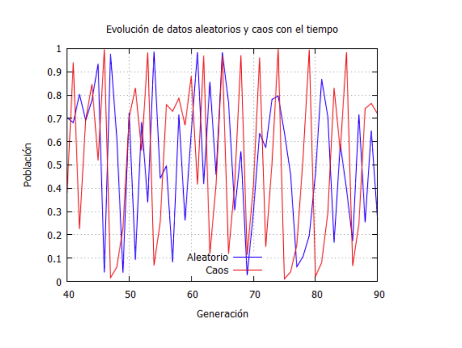
\includegraphics[width=6cm, height=6cm]{Im8.png}
\end{center}

Se puede observar que la linea azul representa datos aleatorios, mientras la roja muestra un crecimiento logístico de 3.99, que corresponde a caos determinista. Se puede hacer un diagrama de fase para diferenciarlos.

\begin{center}
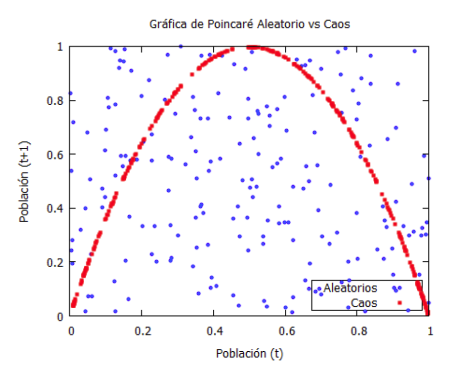
\includegraphics[width=6cm, height=6cm]{Im9.png}
\end{center}

\section{El efecto mariposa}

Los sistemas caóticos muestran la peculiaridad de que son muy sensibles a los cambios en sus condiciones iniciales. Los puntos cercanos divergen con el tiempo. Si los pequeños errores de los parámetros inciales no son dados debido a la impresición, se hacen grandes cambios conforme pasa el tiempo, esto es un reflejo de la vida real.

Se puede observar que conforme pasa el tiempo, las siguientes lineas divergen. Esto es conocido como el efecto mariposa.

\begin{center}
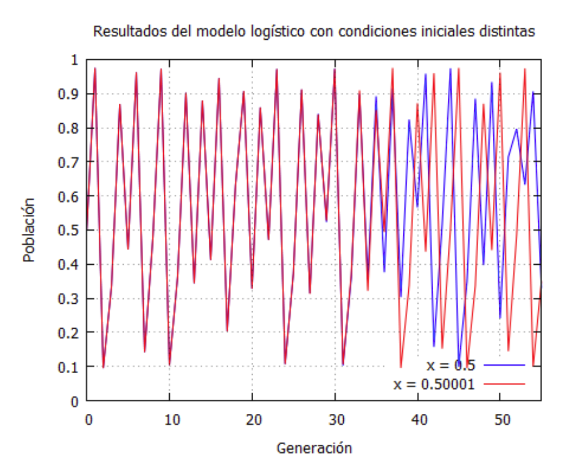
\includegraphics[width=6cm, height=6cm]{Im10.png}
\end{center}

\section{implicaciones del caos}

Los sistemas caóticos y fractales del mundo real incluyen grifos con fugas, helechos, frecuencias cardíacas y generadores de números aleatorios. Muchos estudiosos han estudiado las implicaciones de la teoría del caos para las ciencias sociales, las ciudades y la planificación urbana. El caos indica fundamentalmente que existen límites para el conocimiento y la predicción. Algunos futuros pueden ser desconocidos con precisión. Los sistemas deterministas pueden producir un comportamiento salvajemente fluctuante y no repetitivo. Las intervenciones en un sistema pueden tener resultados impredecibles, incluso si inicialmente cambian las cosas solo ligeramente, ya que estos efectos se combinan con el tiempo.


\section{conclusión}

El estudio de sistemas caóticos es posible haciendo uso de las aseveraciones correspondientes. El uso de máxima para estudiar este tema es de gran utilidad y de fácil manipulación.

\section{Bibliografía}

http://geoffboeing.com/2015/03/chaos-theory-logistic-map/

\end{document}
